% \iffalse
\let\negmedspace\undefined
\let\negthickspace\undefined
\documentclass[journal,12pt,twocolumn]{IEEEtran}
\usepackage{cite}
\usepackage{amsmath,amssymb,amsfonts,amsthm}
\usepackage{algorithmic}
\usepackage{graphicx}
\usepackage{textcomp}
\usepackage{xcolor}
\usepackage{txfonts}
\usepackage{listings}
\usepackage{enumitem}
\usepackage{mathtools}
\usepackage{gensymb}
\usepackage{comment}
\usepackage[breaklinks=true]{hyperref}
\usepackage{tkz-euclide} 
\usepackage{listings}
\usepackage{gvv}                            \usepackage{tikz}
\usepackage{circuitikz}
\def\inputGnumericTable{}                                
\usepackage[latin1]{inputenc}                            
\usepackage{color}                                       
\usepackage{array}                                       
\usepackage{longtable}                                   
\usepackage{calc}                              
\usepackage{tikz}
\usepackage{multirow}                                    
\usepackage{hhline}                                      
\usepackage{ifthen}                            
\usepackage{caption}
\usepackage{lscape}
\usepackage{amsmath}
\newtheorem{theorem}{Theorem}[section]
\newtheorem{problem}{Problem}
\newtheorem{proposition}{Proposition}[section]
\newtheorem{lemma}{Lemma}[section]
\newtheorem{corollary}[theorem]{Corollary}
\newtheorem{example}{Example}[section]
\newtheorem{definition}[problem]{Definition}
\newcommand{\BEQA}{\begin{eqnarray}}
\newcommand{\EEQA}{\end{eqnarray}}
\newcommand{\define}{\stackrel{\triangle}{=}}
\theoremstyle{remark}
\newtheorem{rem}{Remark}

\begin{document}

\bibliographystyle{IEEEtran}
\vspace{3cm}

\title{NCERT Math 11.9.2 Q8}
\author{EE23BTECH11009 - AROSHISH PRADHAN$^{*}$% <-this % stops a space
}
\maketitle
\newpage
\bigskip
\textbf{Question:} An input voltage in the form of a square wave of frequency $1\, kHz$ is given to a circuit, which results in the output shown schematically below. Which one of the following options is the CORRECT representation of the circuit?

\begin{figure}[!h]
    \centering
    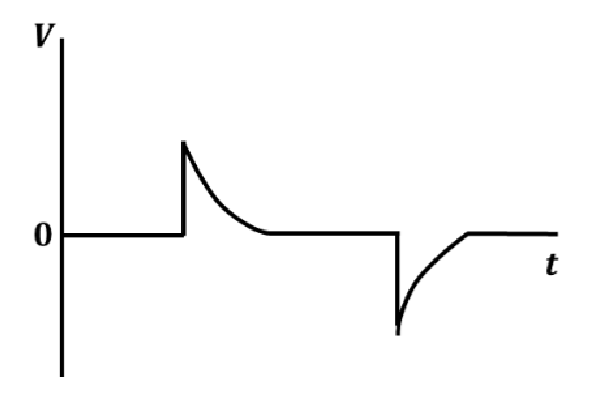
\includegraphics[width = 0.6\columnwidth]{figs/question.png}
    \caption{}
    \label{fig:ques_gate.ph.23.37}
\end{figure}

\begin{enumerate}[label = (\alph*)]
    \item 
    \begin{figure}[!h]
        \centering
        \resizebox{0.2\textwidth}{!}{\begin{circuitikz}
    \draw(0, 0) to[short,*-*] ++ (4,0);
\draw (0,2) to[C,l=$0.1\mu F$, *-*] ++ (3,0) coordinate(a);
\draw (a) to[short,-*] ++ (1,0);
\draw (a) to[R, l_=$0.5k\Omega$,*-] ++(0,-2);

% Voltage labels
\draw (0,2) to[open,l_=V$_{in}$] ++(0,-2);
\draw (4,2) to[open,l=V$_{out}$] ++(0,-2);
\end{circuitikz}

}
        \label{optA_gate.ph.23.37}
    \end{figure}

    \item 
    \begin{figure}[!h]
        \centering
        \resizebox{0.2\textwidth}{!}{\begin{circuitikz}
    \draw(0, 0) to[short,*-*] ++ (4,0);
\draw (0,2) to[C,l=$1\mu F$, *-*] ++ (3,0) coordinate(a);
\draw (a) to[short,-*] ++ (1,0);
\draw (a) to[R, l_=$5k\Omega$,*-] ++(0,-2);

% Voltage labels
\draw (0,2) to[open,l_=V$_{in}$] ++(0,-2);
\draw (4,2) to[open,l=V$_{out}$] ++(0,-2);
\end{circuitikz}

}
        \label{optB_gate.ph.23.37}
    \end{figure}

    \item 
    \begin{figure}[!h]
        \centering
        \resizebox{0.2\textwidth}{!}{\begin{circuitikz}
    \draw(0, 0) to[short,*-*] ++ (4,0);
\draw (0,2) to[R, l = $0.5k\Omega$, *-] ++ (3,0) coordinate(a);
\draw (a) to[short,-*] ++ (1,0);
\draw (a) to[C,l_=$0.1\mu F$,*-*] ++(0,-2);

% Voltage labels
\draw (0,2) to[open,l_=V$_{in}$] ++(0,-2);
\draw (4,2) to[open,l=V$_{out}$] ++(0,-2);
\end{circuitikz}

}
        \label{optC_gate.ph.23.37}
    \end{figure}

    \item 
    \begin{figure}[!h]
        \centering
        \resizebox{0.2\textwidth}{!}{\begin{circuitikz}
    \draw(0, 0) to[short,*-*] ++ (4,0);
\draw (0,2) to[R, l = $5k\Omega$, *-] ++ (3,0) coordinate(a);
\draw (a) to[short,-*] ++ (1,0);
\draw (a) to[C,l_=$1\mu F$,*-*] ++(0,-2);

% Voltage labels
\draw (0,2) to[open,l_=V$_{in}$] ++(0,-2);
\draw (4,2) to[open,l=V$_{out}$] ++(0,-2);
\end{circuitikz}

}
        \label{optD_gate.ph.23.37}
    \end{figure}
\end{enumerate}

\solution
\begin{table}[!h]
    \centering
    \begin{tabular}{|c|c|c|}
    \hline
       \textbf{Symbol}  & \textbf{Value} &  \textbf{Description}\\
    \hline
       $V_{in}$  &  &  Input Voltage\\
    \hline
        $V_{out}$ & & Output Voltage\\
    \hline
        $f$ & $1000Hz$ & Input Wave Frequency\\
    \hline
        $T$ & $\dfrac{1}{f} = 10^{-3} s$ & Input Wave Time Period\\
    \hline
        \multirow{4}{*}{$R$} & (a) $0.5k\Omega$ & \multirow{4}{*}{Resistance}\\
        \cline{2-2}
        & (b) $5k\Omega$ &\\
        \cline{2-2}
        & (c) $0.5k\Omega$ &\\
        \cline{2-2}
        & (d) $5k\Omega$ &\\
    \hline
        \multirow{4}{*}{$C$} & (a) $0.1\mu F$ & \multirow{4}{*}{Capacitance}\\
        \cline{2-2}
        & (b) $1\mu F$ &\\
        \cline{2-2}
        & (c) $0.1\mu F$ &\\
        \cline{2-2}
        & (d) $1\mu F$ &\\
    \hline
        $\tau$ & $RC$ & Time Constant\\
    \hline
    \end{tabular}
    \caption{Given Parameters}
    \label{tab:1_gate.23.ph.37}
\end{table}

When rising edge of square waveform is applied, capacitor is at discharged state:
\begin{align}
    \therefore V_C = 0
\end{align}
at rising edge.

$\therefore$ options (c) and (d) are wrong.

Time constants ($\tau$) of circuits (a) and (b) are given below:
\begin{table}[!h]
    \centering
    \begin{tabular}{|c|c|}
    \hline
       $s_k$  &  \textbf{Value}\\
    \hline
       $s_0$  & $-0.162 + 1.003j$\\
    \hline
       $s_1$  & $-0.391 + 0.415j$\\
    \hline
       $s_2$  & $-0.391 - 0.415j$\\
    \hline
       $s_3$  & $-0.162 - 1.003j$\\
    \hline
    \end{tabular}
    \caption{Poles on left half of complex plane}
    \label{tab:2}
\end{table}

\begin{align}
    \because 5\tau_{(a)} = 2.5\times 10^{-4}< T = 10^{-3}
\end{align}
the capacitor charges (i.e. $V_{out} = 0$) before the next wave cycle.

$\therefore$ option (a) is correct.

\begin{figure}[!h]
    \centering
    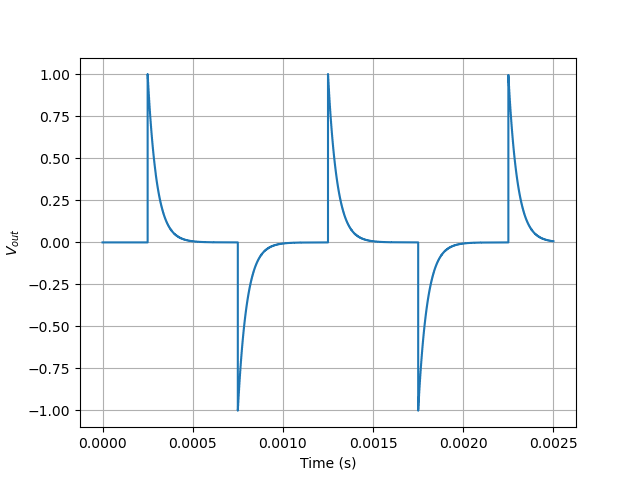
\includegraphics[width = \columnwidth]{figs/assign4.png}
    \caption{Response of circuit (a) for $R = 0.5k\Omega$, $C = 0.1\mu F$, $f = 1000Hz$ and $V_{in, max} = 1V$}
    \label{fig:enter-label}
\end{figure}
\end{document}

